\documentclass{astroedu-lab}

\begin{document}

\pagestyle{plain}

\begin{problem}{\huge Лабораторная работа 4.1.1(2)\\\\Изучение центрированных оптических систем\\\\Моделирование оптических приборов и определение их увеличения\\\\Геометрическая оптика\\\\Выполнил Жданов Елисей Б01-205}

\section{Цель работы:}

1) Изучить методы определения фокусных расстояний
линз и сложных оптических систем; определить характеристики оптической системы, составленной из тонких линз; изучить недостатки
реальных линз - сферическую и хроматическую аберрации.

2) Изучить модели зрительных труб (астрономической
трубы Кеплера и земной трубы Галилея) и микроскопа, определить
их увеличения.

\section{Оборудование:}

1) Оптическая скамья с набором рейтеров

2) Положительные и отрицательные линзы

3) Экран

4) Осветитель с ирисовой диафрагмой

5) Зрительная труба

6) Светофильтры

7) Кольцевые диафрагмы

8) Линейка

\section{Теоретическая справка}

\subsection*{Определения фокусных расстояний}
Формула тонкой линзы имеет вид
\begin{equation}
    \frac{1}{f} = \frac{1}{a} + \frac{1}{b},
\end{equation}
\noindent
где $f$ -- фокусное расстояние, $a$ -- расстояния от предмета до линзы, $b$ -- расстояние от изображения до линзы.

\noindent
Для измерения фокусного расстояния тонкой собирающей линзы может использоваться схема с рис. 1. и формула (2).
\begin{equation}
    f = \frac{L^2 - l^2}{4L}
\end{equation}

\begin{figure}[H]
    \centering
    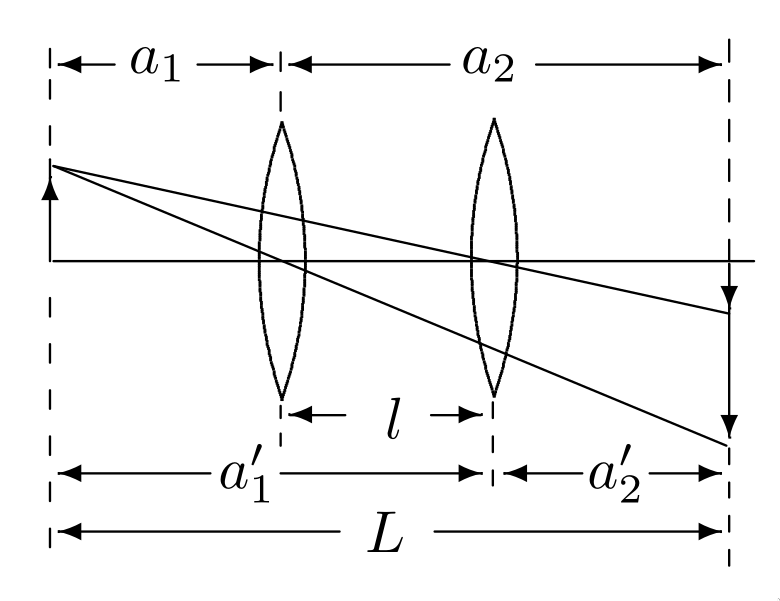
\includegraphics[scale=0.3]{pic_1.png}
    \caption{Схема измерения фокуса тонкой собирающей линзы}
\end{figure}

\noindent
Также фокусное расстояние тонкой собирабщей линзы можно измерить с помощью зрительной трубы, настроенной на бесконечность. Если расположить линзу между предметом и трубой и найти четкое изображение предмета, то расстояние от линзы до предмета будет равно фокусному.

\noindent
Для определения расстояние тонкой рассеивающей линзы поспользуемся схемой на рис. 2 и формулой тонкой линзы. Также можно восползоваться зриетльной трубой, настроенной на бесконечность. Если расположить предмет у нее в фокусе, то изображение переместиться в бесконечность, что можно проверить с помощью зрительной трубы.

\begin{figure}[H]
    \centering
    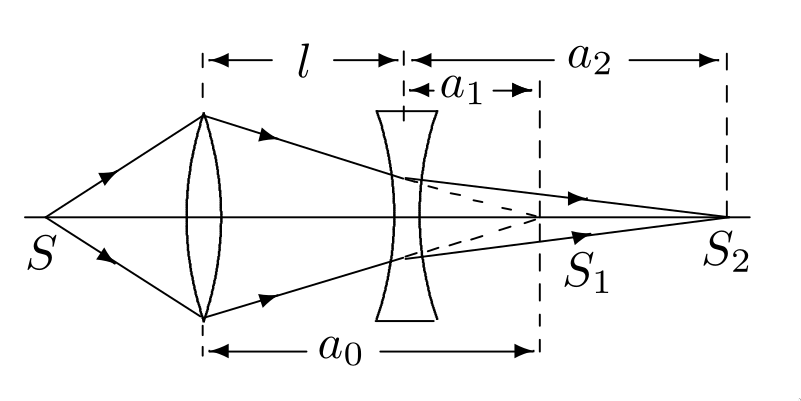
\includegraphics[scale=0.35]{pic_2.png}
    \caption{Схема измерения фокуса тонкой рассеивающей линзы}
\end{figure}

\noindent
Для определения фокусного расстояние и положения главных плоскостей сложной оптической системы может использоваться метод Аббе: схема на рис. 3 и формула (3).

\begin{figure}[H]
    \centering
    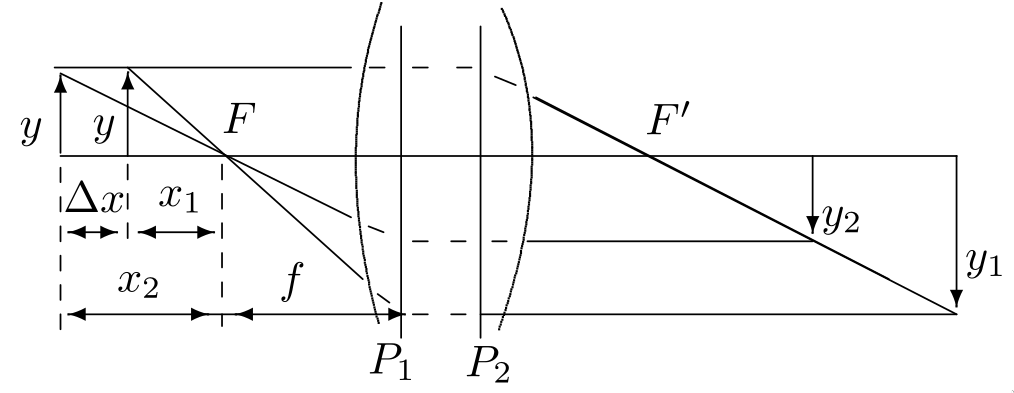
\includegraphics[scale=0.3]{pic_3.png}
    \caption{Схема определения фокусного расстояние и положения главных плоскостей сложной оптической}
\end{figure}

\begin{equation}
    f = \frac{\Delta x}{y / y_1 - y / y_2}    
\end{equation}


\subsection*{Аберрации реальных оптических систем}
Сферическая аберрация -- аберрация, связанная с формой линзы. При прохождении через нее не параксиального пучка лучи, проходящие на разных расстояниях от главной оптической оси собираются в разных точках. Для количечественной оценки сферической аберрации будем пользоваться характеристической кривой сферической аберрации, то есть зависимостью 
\begin{equation}
    \delta s(h) = s(h) - s(0) = -\frac12 \left( \frac{n}{n - 1} \right)^2 \left( \frac{h}{f} \right)^2 f
\end{equation}
\noindent
При $h = r$ формула (4) определяет продольную сферическую аберрацию. \\
Хроматическая аберрация -- аберрация, связанная с немонохроматичностью проходящего через линзу света. Показатель преломления вещества зависит от длины волны падающего света, а значит лучу с разынами длинами волны будут собираться в разных точках. Для количечественной оценки хроматической аберрации воспользуемся соотношениями
\begin{equation}
    \delta f_\text{хр} = f_F - f_C,
\end{equation}
\begin{equation}
    \nu = \frac{n_D - 1}{n_F - n_C},
\end{equation}
\begin{equation}
    \delta f_\text{хр} = -\frac{1}{\nu} f_D,
\end{equation}
\noindent
где $f_F$ -- фоккусное расстояние для длины волны 486.1 нм, $f_C$ -- фокусное расстояние для длины волны 656.3 нм, $f_D$ -- фокусное расстояние для длины волны 589.3 нм, $\nu$ -- число Аббе.


\subsection*{Телескопы}

Для любых телескопических систем, у которых $n=n^{\prime}$, согласно (1.30), (1.18) угловое увеличение
$$
N_T \equiv \frac{\alpha^{\prime}}{\alpha}=\frac{y}{y^{\prime}}=\frac{f_1^{\prime}}{f_2}=-\frac{f_1}{f_2}
$$

обратно поперечному увеличению и по абсолютной величине равно отношению фокусных расстояний объектива и окуляра. Угловое увеличение $N_T$ в этом случае называют просто увеличением трубы, опуская прилагательное «угловое». Эта величина показывает, во сколько раз угол, под которым виден бесконечно удалённый малый предмет в трубу, больше угла, под которым он был бы виден невооружённым глазом (рис. 1.8a).

\subsection*{Микроскопы}

Теоретические сведения. Обозначения: $f_{\text {об }}$ - фокус объектива, $f_{\text {ок }}$ - фокус окуляра, $\Delta$ - оптический интервал (расстояние между задним фокусом объектива и передним фокусом окуляра), $L_{3 \text { р }} \approx 25$ см - расстояние наилучшего зрения (для здорового глаза).
При аккомодации глаза на бесконечность угловое увеличение микроскопа
$$
\gamma_{\infty} \equiv \frac{\operatorname{tg} \alpha_2}{\operatorname{tg} \alpha_0}=\frac{y_1 / f_{\text {ок }}}{y_0 / L_{\text {зр }}}=\frac{L_{\text {зр }}}{f_{\text {ок }}} \cdot \frac{\Delta}{f_{\text {об }}}
$$
( $y_0$ - размер предмета, $y_1$ - размер промежуточного изображения предмета в объективе).
При аккомодации глаза на расстояние наилучшего зрения $d_{\text {зр }}$, когда глаз расположен вплотную к окуляру:
$$
\gamma_{\text {зр }}=\frac{y_2 / L_{\text {зр }}}{y_0 / L_{\text {зр }}}=\frac{L_{\text {зр }}+f_{\text {ок }}}{f_{\text {ок }}} \frac{\Delta}{f_{\text {об }}}
$$
(в этом случае угловое увеличение совпадает с линейным). При $f_{\text {ок }} \ll L_{\text {зр }}$ формулы совпадают: $\gamma_{\text {зр }} \approx \gamma_{\infty}$.

Изображение предмета в микроскопе можно сделать действительным и сфокусировать его на экране за окуляром (проекционный микроскоп). Увеличение проекционного микроскопа равно
$$
\gamma_{\text {пр }}=\frac{L-f_{\text {ок }}}{f_{\text {ок }}} \cdot \frac{\Delta}{f_{\text {об }}},
$$

где $L-$ расстояние от окуляра до экрана.

\section{Измерения, Обработка}

\subsection{0. Подготовка к работе}

1) В работе используется 5 линз с порядковыми номерами. В дальнейшем будем использовать такую нумерацию.

Линзы 1-4 собирающие, линза 5 - рассеивающая.

2) Центрируем все используемые оптические элементы.

\subsection{I. Определение фокусных расстояний линз с помощью подзорной трубы}

1) Настроим подзорную трубу на бесконечность

2-4) Проведем замеры фокусных расстояний линз с помощью подзорной трубы и занесем их в таблицу.

\begin{center}
\begin{tabular}{|c|c|c|}
\hline 
№ Линзы & $F_1$, см & $F_2$, см \\
\hline
1 & 7.5 & 7.3 \\
2 & 15.0 & 14.5 \\
3 & 19.8 & 20.2 \\
4 & 29.0 & 29.8 \\
\hline
\end{tabular}
\end{center}

Погрешность каждого измерения подразумевается равной 0.1 см.

Судя по результатам измерений, тонкими линзы считать нельзя.

5) Для первой линзы дополнительно проведем измерения с учетом погрешностей

\begin{center}
\begin{tabular}{|c|c|c|c|c|c|}
\hline 
\multicolumn{6}{|c|}{Фокусное расстояние I линзы} \\
\hline
7.5 & 7.3 & 7.4 & 7.3 & 7.6 & 7.4 \\
\hline
\end{tabular}
\end{center}

Грубо усредняя полученные значения, получим результат

\begin{equation}
	F = 7.42 \pm 0.05 \text{ см}
\end{equation}

6) Измерения фокусного расстояния рассеивающей линзы 5 

$a_0 = 17.0 \pm 0.1$ см, $l = 8.4 \pm 0.1$ см. Тогда $f = l - a_0 = -8.6 \pm 0.2$ см.

\subsection{II. Измерение фокусных расстояний линз по формуле тонкой линзы и методом Бесселя}

Проведу измерения для линз I и II.

\subsubsection{I линза}

1) $L = 34.5 \pm 0.1$ см.

2) Расстояния $s_1 = 10.5 \pm 0.1$ см и $s_2 = 23.4 \pm 0.1$ см.

Разность $l = s_2 - s_1 = 12.9 \pm 0.2$ см.

3) По формуле тонкой линзы:

\begin{equation}
	f(s_i) = \left( \frac{1}{s_i} + \frac{1}{L-s_i} \right) ^{-1}
\end{equation}

\begin{equation}
	f(s_1) = 7.30 \pm 0.05 \text{ см}
\end{equation}

\begin{equation}
	f(s_1) = 7.53 \pm 0.08 \text{ см}
\end{equation}

По приближённой формуле Бесселя:

\begin{equation}
	f = \frac{L^2 - l^2}{4 L} = 7.42 \pm 0.07 \text{ см}
\end{equation}

Результаты получились логичные, формула Бесселя эффективно усредняет значения 2-х $s_i$. 

4) Для развернутой линзы

Расстояния $s_1 = 11.0 \pm 0.1$ см и $s_2 = 24.1 \pm 0.1$ см.

Разность $l = s_2 - s_1 = 13.1 \pm 0.2$ см.

По формуле тонкой линзы:

\begin{equation}
	f(s_i) = \left( \frac{1}{s_i} + \frac{1}{L-s_i} \right) ^{-1}
\end{equation}

\begin{equation}
	f(s_1) = 7.49 \pm 0.05 \text{ см}
\end{equation}

\begin{equation}
	f(s_1) = 7.26 \pm 0.09 \text{ см}
\end{equation}

По приближённой формуле Бесселя:

\begin{equation}
	f = \frac{L^2 - l^2}{4 L} = 7.38 \pm 0.07 \text{ см}
\end{equation}

\subsubsection{II линза}

1) $L = 72.4 \pm 0.1$ см.

2) Расстояния $s_1 = 21.2 \pm 0.1$ см и $s_2 = 50.6 \pm 0.1$ см.

Разность $l = s_2 - s_1 = 29.4 \pm 0.2$ см.

3) По формуле тонкой линзы:

\begin{equation}
	f(s_i) = \left( \frac{1}{s_i} + \frac{1}{L-s_i} \right) ^{-1}
\end{equation}

\begin{equation}
	f(s_1) = 14.99 \pm 0.05 \text{ см}
\end{equation}

\begin{equation}
	f(s_1) = 15.20 \pm 0.09 \text{ см}
\end{equation}

По приближённой формуле Бесселя:

\begin{equation}
	f = \frac{L^2 - l^2}{4 L} = 15.12 \pm 0.07 \text{ см}
\end{equation}

Результаты получились логичные, формула Бесселя эффективно усредняет значения 2-х $s_i$. 

4) Для развернутой линзы

Расстояния $s_1 = 21.5 \pm 0.1$ см и $s_2 = 51.4 \pm 0.1$ см.

Разность $l = s_2 - s_1 = 29.9 \pm 0.2$ см.

По формуле тонкой линзы:

\begin{equation}
	f(s_i) = \left( \frac{1}{s_i} + \frac{1}{L-s_i} \right) ^{-1}
\end{equation}

\begin{equation}
	f(s_1) = 15.1 \pm 0.05 \text{ см}
\end{equation}

\begin{equation}
	f(s_1) = 14.9 \pm 0.09 \text{ см}
\end{equation}

По приближённой формуле Бесселя:

\begin{equation}
	f = \frac{L^2 - l^2}{4 L} = 15.01 \pm 0.07 \text{ см}
\end{equation}

Результаты получились логичные, формула Бесселя эффективно усредняет значения 2-х $s_i$.

\subsection{III. Измерение фокусных расстояний методом Аббе}

Проведу измерения для линз I и II.

$y_0 = 2.0 \pm 0.1$ см

\subsubsection{I линза}

1) Занесем измеренные величины в таблицу

\begin{center}
\begin{tabular}{|c|c|c|}
\hline 
$s_1$, см & $L$, см & $y_i$, см \\
\hline
11.5 & 35.0 & 1.4 \\
15.5 & 30.0 & 1.9 \\
13.3 & 30.4 & 2.6 \\
15.7 & 30.0 & 1.8 \\
\hline
\end{tabular}
\end{center}

2) Пересчитаем таблицу в величины смещения $\Delta x$

\begin{center}
\begin{tabular}{|c|c|c|}
\hline 
$\Delta x$, см & $\Delta x'$, см & $y_i$, см \\
\hline
0 & 0 & 1.8 \\
0.2 & 0.2 & 1.9 \\
2.4 & 2.8 & 2.6 \\
\hline
\end{tabular}
\end{center}

3) Фокусные расстояния по формулам Аббе:

$$
f=\frac{\Delta x^{\prime}}{y_1 / y_0-y_2 / y_0}=\frac{\Delta x}{y_0 / y_2-y_0 / y_1} .
$$

и

$$
f^2=\Delta x \cdot \Delta x^{\prime} \cdot \frac{y_2 y_1}{\left(y_2-y_1\right)^2}
$$

$F_{21} = 7 \pm 3$

$F_{22} = 10 \pm 10$ см

$F_{23} = 7 \pm 3$ см

Как видим, точность метода Аббе весьма низка, хотя результаты довольно близки к значениям предыдущего пункта

\subsubsection{II линза}

1) Занесем измеренные величины в таблицу

\begin{center}
\begin{tabular}{|c|c|c|}
\hline 
$s_1$, см & $L$, см & $y_i$, см \\
\hline
27.5 & 61.5 & 2.4 \\
33.3 & 61.1 & 1.6 \\
\hline
\end{tabular}
\end{center}

2) Пересчитаем таблицу в величины смещения $\Delta x$

\begin{center}
\begin{tabular}{|c|c|c|}
\hline 
$\Delta x$, см & $\Delta x'$, см & $y_i$, см \\
\hline
0 & 0 & 1.6 \\
5.8 & 6.2 & 2.4 \\
\hline
\end{tabular}
\end{center}

3) Фокусные расстояния по формулам Аббе:

$F_{21} = 16 \pm 5$

$F_{22} = 14 \pm 5$ см

$F_{23} = 15 \pm 5$ см

Главная причина большой погрешности измерения фокусного расстояния - неточность определения размера изображения. Для улучшения точности необходимо увеличивать смещения $\Delta x$.

\subsection{IV. Сборка и изучение подзорных труб Кеплера и Галилея}

1) Выберем 2 линзы I и II и оптическую схему Кеплера.

Теоретическое увеличение телескопа $\gamma_{\text{теор}} = \frac{f_{II}}{f_I} = 2.02 \pm 0.03$.

В качестве коллиматора будем использовать линзу IV.

2) Установим транспарант в фокус коллиматорной линзы.

3-5) Фотографии

\begin{figure}[H]
    \centering
    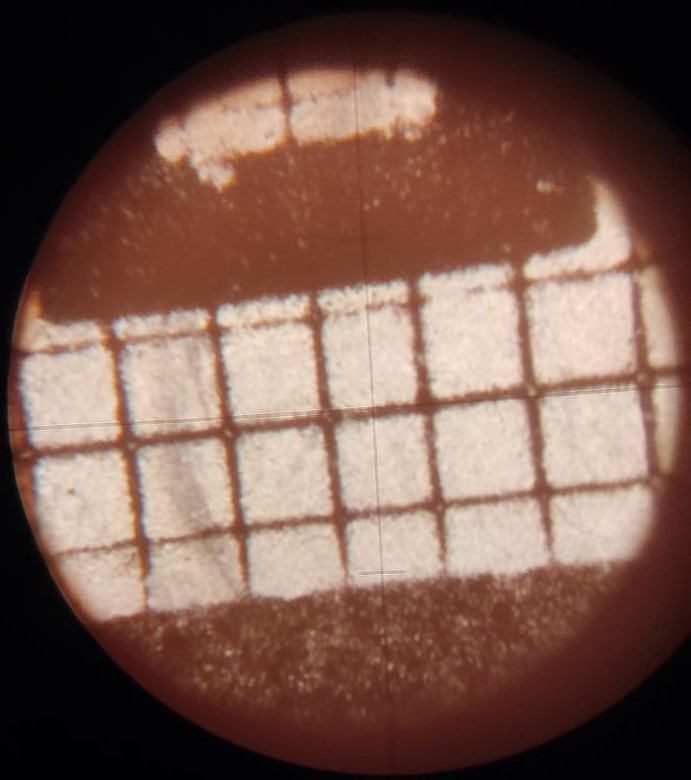
\includegraphics[scale=0.35]{7.jpg}
    \caption{Фотография источника без увеличения}
\end{figure}

\begin{figure}[H]
    \centering
    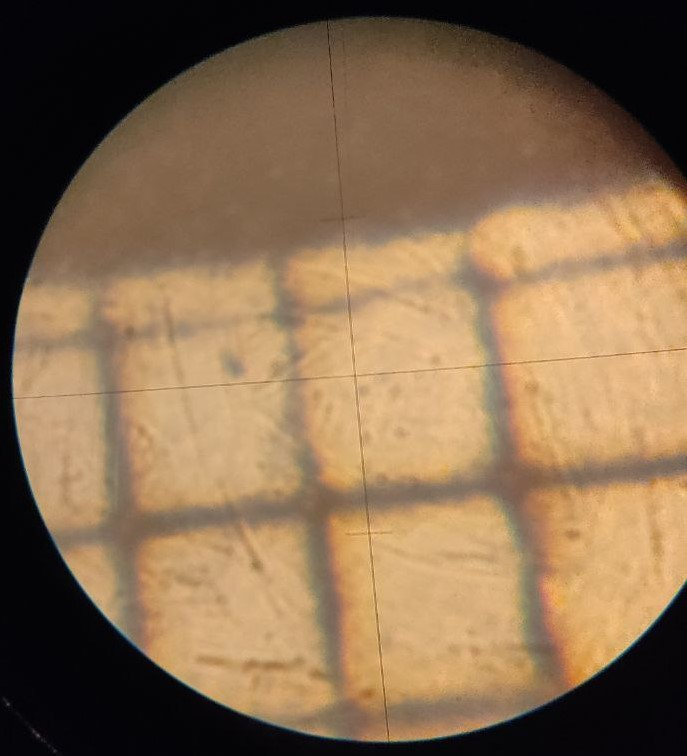
\includegraphics[scale=0.35]{3.jpg}
    \caption{Фотография источника через телескоп}
\end{figure}

6) Усредняя размеры сторон 5 клеток около центра изображения, получим размер клетки в $93.6 \pm 1.5$ пиксела.

На втором изображении через телескоп размер клетки составляет $181 \pm 3$

Наконец, практическое увеличение составит $\gamma_{\text{эксп}} = \frac{px_2}{px_1} = 1.93 \pm 0.06$, что совпадает с теоретическим расчетом в рамках погрешности.

7) Измерим диаметры зрачков входного и выходного пучка

$D = 5.1$ см, $d = 2.5$ см. Тогда $\gamma_{\text{зрач}} = \frac{D}{d} = 2.04 \pm 0.13$.

Такой результат нас вполне устраивает.

\subsection{V. Сборка и изучение модели микроскопа}

Выберем линзы I и II.

1) Выразим оптический интервал как функцию фокусных расстояний и увеличения

\begin{equation}
	\Delta = \frac{\gamma f_1 f_2}{L} = 17.8 \text{ см}
\end{equation}

Тогда расстояние между линзами $l_{12} = \Delta + f_1 + f_2 = 40.2 \text{ см}$

2) Соберем схему в соответствии с рассчетами.

3) Фотография измерений с помощью зрительной трубы

\begin{figure}[H]
    \centering
    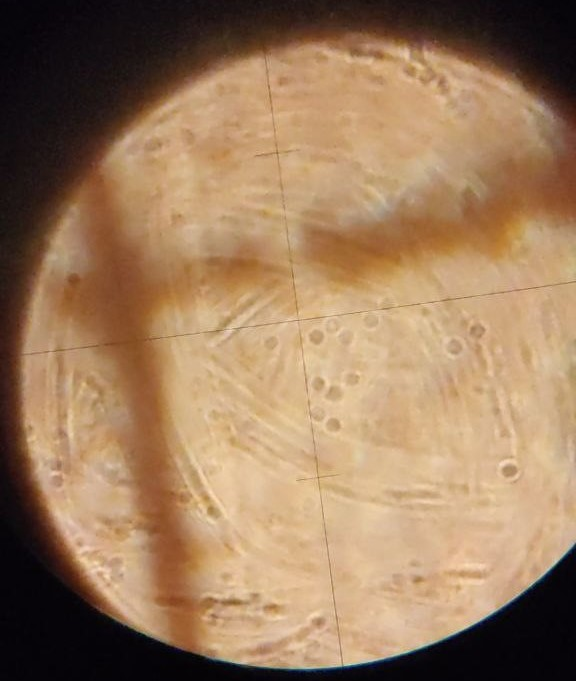
\includegraphics[scale=0.35]{1.jpg}
    \caption{Фотография источника через телескоп}
\end{figure}

Более тчательный анализ с помощью видеоряда дал результат $420 \pm 20 $ пикселов. Итоговое увеличение $\gamma_\text{эксп} = 4.5 \pm 0.3$. Используя формулу для пересчета увеличения в режиме аккомодации на бесконечность

\begin{equation}
	\gamma_{\infty} = \frac{\alpha}{\alpha_0} \cdot \frac{L_\text{ зр}}{f_\text{кол}} = 4.4 \pm 0.3
\end{equation}

что входит в пределы теоретического значения.

\subsection{VI. Изучение составной оптической системы}

В пункте были использованы собирающая линза I и рассеивающая линза V.

1) Поскольку оптическая сила положительной линзы больше, система фокусирующая. Проверим это

Расстояние между линзами $l = 5.1 \pm 0.1$ см

Фокусное расстояние системы

\begin{equation}
	f = \left( \frac{1}{f_1} + \frac{1}{f_2} - \frac{l}{f_1 f_2} \right) = 10.2 \pm 0.4 \text{ см} > 0
\end{equation}

2) Расстояние от ближайшей линзы до фокуса(источника) $s_1 = 15.5$ см. Расстояние с другой стороны точно измерить не получилось, оно оказалось чуть меньше 6 см.

3) Занесем в табличу смещение и расстояние между экраном и источником

\begin{center}
\begin{tabular}{|c|c|}
\hline 
L, см & l, см \\
\hline
56.5 & 24.2 \\
53.0 & 17.4 \\
51.0 & 22.0 \\
47.0 & 6.2 \\
60.0 & 27.5 \\
64.0 & 32.6 \\
\hline
\end{tabular}
\end{center}

Используя линеаризацию параболой(квадратичная), получим коэффициенты кривой $l^2 = y = x^2 - (2 \delta + 4 f) x + \delta (\delta + 4 f)$

Получим

$c x^2 = 1 x^2$ - фиксируем с равное 1

Возьмем $y = l^2 - L^2$, а $x = L$

\newpage

Построим зависимость $y(x)$

\begin{center}
	\Large $y(x)$
\end{center}

\begin{figure}[H]
    \centering
    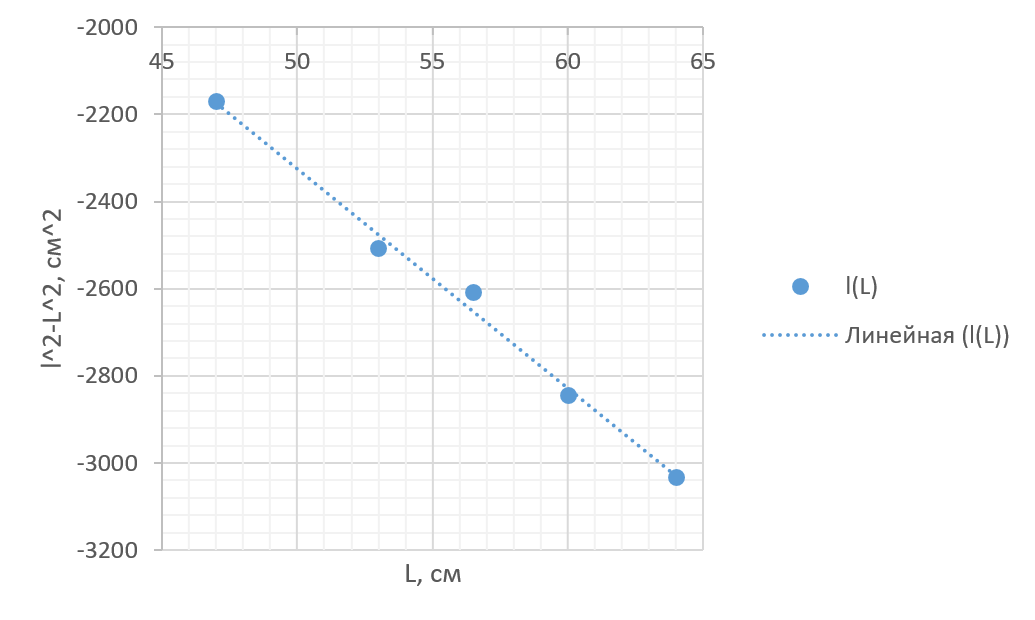
\includegraphics[scale=0.45]{2024-04-08_01-52-45}
\end{figure}

Найдем угловые коэффициенты прямых для каждой установки по МНК.

\[
	a = \frac{<x_i y_i> - < x > < y_i >}{< x_i^2> - < x_i >^2}
\]

\[
	b = < \nu_i > - a < N_i >
\]

Также рассчитаем их погрешности

\begin{equation}
	S_a^2 = \frac{< x_i^2>}{< x_i^2 > - < x_i >^2} \cdot \frac{<  b_i - b > ^2}{n - 2}
\end{equation}

$-(2 \delta + 4 f) x = -(50.4 \pm 2.5) x$

$\delta (\delta + 4 f) = 190 \pm 140$

Оценим из этих отношений $\delta$ и $f$.

$\delta = 46 \pm 4$ см

$f = 10.4 \pm 1.9$ см.

Данное значение очень хорошо согласуется с теорией.


%\begin{center}
%\begin{tabular}{|c|c|c|c|}
%\hline 
%\multicolumn{2}{|c|}{$h_\text{ман}$, мм} & $\sigma, \frac{\text{мН}}{\text{К}}$ & T, $^\circ$C \\
%\hline
%188.0 & 188.0 & $(64.5 \pm 3.9)$ & 22\\
%187.0 & 187.0 & $(64.0 \pm 3.9)$ & 30\\
%185.5 & 186.0 & $(63.3 \pm 3.9)$ & 35\\
%184.0 & 184.5 & $(62.5 \pm 3.9)$ & 40\\
%182.5 & 183.0 & $(61.7 \pm 3.9)$ & 45\\
%181.0 & 181.0 & $(60.8 \pm 3.8)$ & 50\\
%179.0 & 179.5 & $(59.9 \pm 3.8)$ & 55\\
%177.5 & 177.5 & $(59.0 \pm 3.8)$ & 60\\
%\hline
%\end{tabular}
%\end{center}
%
%
%Найдем угловые коэффициенты прямых для каждой установки по МНК.
%
%\[
%	a = \frac{<x_i y_i> - < x > < y_i >}{< x_i^2> - < x_i >^2}
%\]
%
%\[
%	b = < \nu_i > - a < N_i >
%\]
%
%Также рассчитаем их погрешности
%
%\begin{equation}
%	S_a^2 = \frac{< x_i^2>}{< x_i^2 > - < x_i >^2} \cdot \frac{<  b_i - b > ^2}{n - 2}
%\end{equation}
%
%
%\begin{center}
%	\Large $q(T)$
%\end{center}

%\begin{figure}[!h]
%	\centering
%	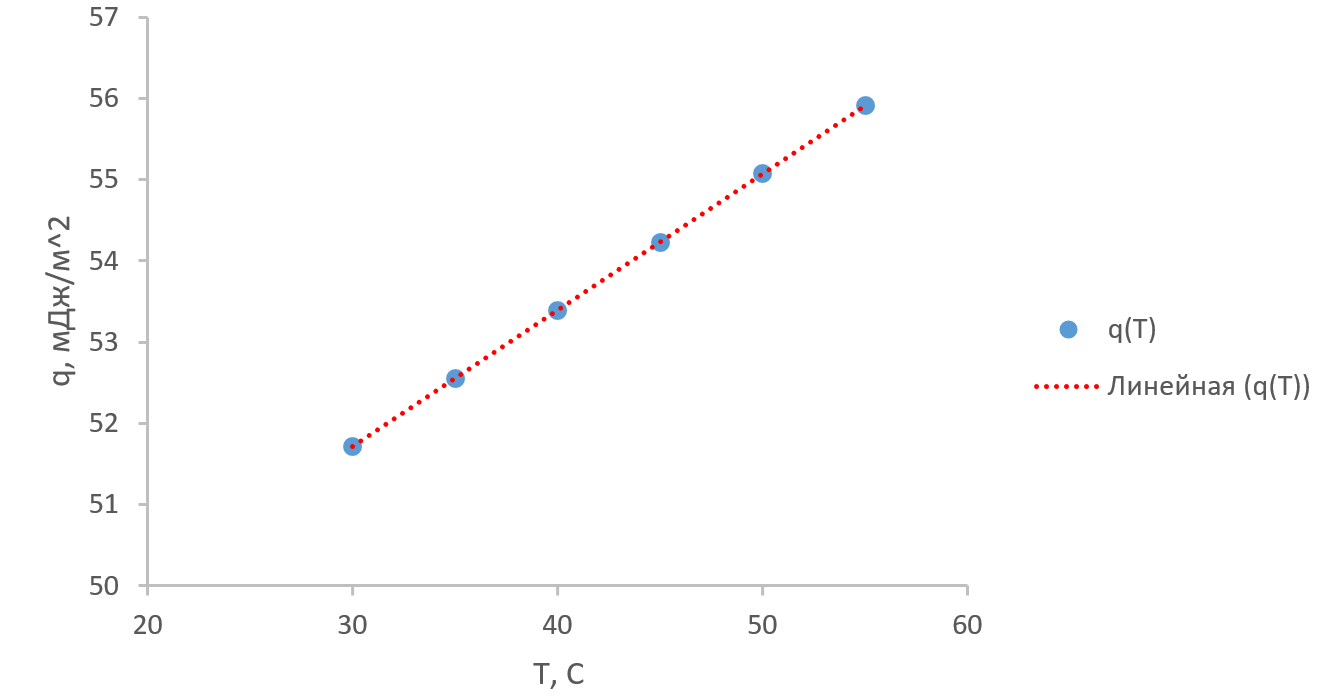
\includegraphics[width=1\textwidth]{2023-02-23_22-23-59.png}
%	\label{fig:boiler}
%\end{figure}

\section{Вывод}

Сравнивая результаты метода Бесселя и Аббе, можно с увереностью сказать, что автор, привыкший постоянно использовать в жизни первый метод, получает им лучший результат, что совершенно не порочит второй подход. Просто в данной работе довольно сложно изменять величины в больших пределах, поэтому метод Бесселя дал более доверительные результаты.

В целом, в работе постоянно использовалась диафрагма для нивелирования аберраций.

Что касается оптических схем, все они были успешно реализованы и дали разумные результаты.

\section{Ресурсы}

Расчет по МНК: метод-наименьших-квадратов.рф


\end{problem}
\end{document}